\chapter{Anexo I: Árbol de Problema }

\begin{figure}[h]
	\begin{center}
		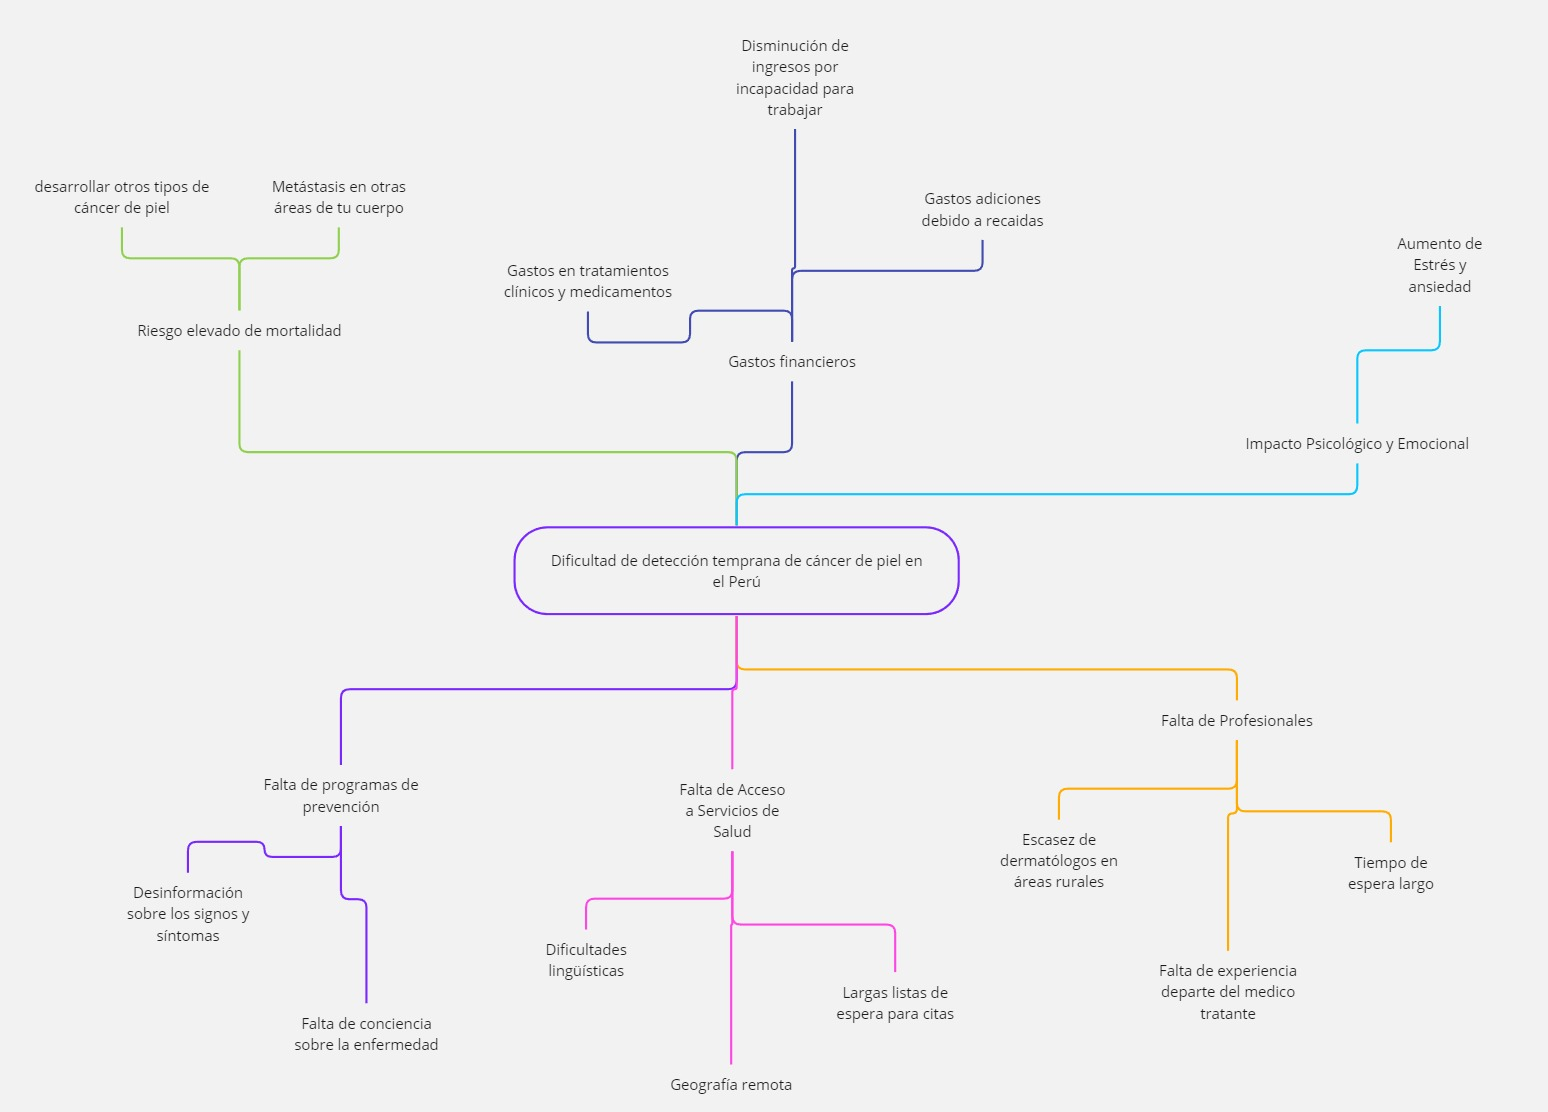
\includegraphics[width=0.8\textwidth]{images_repo/Anexo/Problem Tree Template.jpg}
		\caption{Árbol de Problema. Fuente: Elaboración propia}
		\label{1:arbolProblema}
	\end{center}
\end{figure}



\chapter{Anexo II: Árbol de Objetivo}

\begin{figure}[h]
	\begin{center}
		\includegraphics[width=0.8\textwidth]{images_repo/Anexo/Árbol de Objetivos.jpg}
		\caption{Árbol de Problema. Fuente: Elaboración propia}
		\label{1:arbolObjeti}
	\end{center}
\end{figure}



\chapter{Anexo II: Matriz de Consistencia}


\begin{table}[h!]
	\centering
	\small
	\begin{tabular}{ |m{5cm}|m{5cm}|m{5cm}|  }
		\hline
		\rowcolor{bluejean}
		\Centering \color{white}{PROBLEMAS}& \Centering \color{white}{OBJETIVOS}& \Centering \color{white}{HIPÓTESIS}\\
		\hline
		\rowcolor{turq}
		\Centering Problema General& \Centering Objetivo General & \Centering Hipótesis General \\
		\hline
		{\ProblemaGeneral} & { \ObjetivoGeneral} & {\HipotesisGeneral} \\
		\hline
		\rowcolor{turq}
		\Centering Problemas Específicos& \Centering Objetivos Específicos & \Centering Hipótesis Específicas \\
		\hline
		{\Pbone} & {\Objone} & {\Hone} \\
		\hline
		{\Pbtwo} & {\Objtwo} & {\Htwo} \\
		\hline
		{\Pbthree} & {\Objthree} & {\Hthree} \\
		\hline
		{\Pbfour} & {\Objfour} & {\Hfour} \\
		\hline
		{\Pbfive} & {\Objfive} & {\Hfive} \\
		\hline
	\end{tabular}
	\caption{Matriz de consistencia. Fuente: Elaboración propia}
	\label{1:table}
\end{table}



\chapter{Anexo II: Resumen de Papers investigados}
%\section{Conclusiones}

\begin{table}[h]
	\newcommand{\multirot}[1]{\multirow{2}{*}[-8ex]{\rotcell{\rlap{#1}}}}
	%\scriptsize
	\footnotesize
	\centering
	\begin{tabular}{|m{0.5cm}|m{0.3cm}|m{4cm}|m{2cm}|m{0.6cm}|m{1.7cm}|m{3cm}|} 
		\hline
		\rowcolor[rgb]{0,0.251,0.502} \multicolumn{1}{|c|}{\textcolor{white}{Tipo}} & \multicolumn{1}{c|}{\textcolor{white}{N°}} & \multicolumn{1}{c|}{\textcolor{white}{Título}}                                                                             & \multicolumn{1}{c|}{\textcolor{white}{Autor}}        & \multicolumn{1}{c|}{\textcolor{white}{Año}} & \multicolumn{1}{c|}{\textcolor{white}{País}} & \multicolumn{1}{c|}{\textcolor{white}{Fuente}}                                                        \\ 
		\hline
		\multirot{Problema}                                        & 1                                             & Copper price estimation using bat algorithm~                                                                               & Dehghani  Bogdanovic                                 & 2018                                        & United Kingdom                               & Resources Policy                                                                                      \\ 
		\cline{2-7}
		& 2                                             & Alternative techniques for forecasting mineral commodity prices                                                            & Cortez, Saydam, Coulton,  Sammut                     & 2018                                        & Netherlands                                  & International Journal of Mining Science and Technology                                                \\ 
		\hline
		\multirow{3}{*}[-14ex]{\rotcell{\rlap{Propuesta}}}
		& 3                                             & Prediction of the crude oil price thanks to natural language
		processing applied to newspapers~                           & Trastour, Genin,  Morlot                             & 2016                                        & USA                                          & Standfort University ML repository                                                                    \\ 
		\cline{2-7}
		& 4                                             & Stock Price Prediction Using Deep Learning~                                                                                & Tipirisetty                                          & 2018                                        & USA                                          & Master's Theses San Jose State University                                                             \\ 
		\cline{2-7}
		& 5                                             & Deep Learning for Stock Prediction Using Numerical and Textual
		Information                                               & Akita, R., Yoshihara, A., Matsubara, T.,  Uehara, K. & 2016                                        & USA                                          & 2016 IEEE/ACIS 15th International Conference on Computer and
		Information Science (ICIS)             \\ 
		\hline
		\multirow{4}{*}[-28ex]{\rotcell{\rlap{Técnica}}}                                          & 6                                             & Stock Prices Prediction using the Title of Newspaper Articles
		with Korean Natural Language Processing~                   & Yun, Sim,  Seok                                      & 2019                                        & Japan                                        & 2019 International Conference on Artificial Intelligence in
		Information and Communication (ICAIIC)  \\ 
		\cline{2-7}
		& 7                                             & A Method of Optimizing LDA Result Purity Based on Semantic
		Similarity                                                    & Jingrui, Z., Qinglin, W., Yu, L.,  Yuan, L.          & 2017                                        & China                                        & 2017 32nd Youth Academic Annual Conference of Chinese
		Association of Automation (YAC)~              \\ 
		\cline{2-7}
		& 8                                             & Qualitative Stock Market Predicting with Common Knowledge Based
		Nature Language Processing: A Unified View and Procedure & Rao, D., Deng, F., Jiang, Z.,  Zhao, G.~             & 2015                                        & USA                                          & 2015 7th International Conference on Intelligent Human-Machine
		Systems and Cybernetics              \\ 
		\cline{2-7}
		& 9                                             & Fuzzy Bag-of-Words Model for Document Representation                                                                       & Zhao, R.,  Mao, K.                                   & 2018                                        & USA                                          & IEEE Transactions on Fuzzy Systems (~Volume:
		26~,~Issue: 2~, April 2018~)                           \\
		\hline
	\end{tabular}
	\caption{Cuadro Resumen de Papers investigados. Fuente: Elaboración propia}
\label{A:table}
\end{table}




